%==========================================================================
% BEGIN #4 - CONCEÇAO DO SISTEMA DE DADOS
% Descrição e caracterização geral do sistema responsável pelo armazenamento da informação requerida pelo sistema que idealizaram e especificaram.
%==========================================================================

\chapter{Conceção do Sistema de Dados}
    Os requisitos exigem acesso tanto a um catálogo de modelos e peças como a um registo de utilizadores da aplicação, que a usam para assinalar a sua autoria na conceção de encomendas. Com isto em mente, partiu-se do diagrama estrutural de domínio para estabelecer como os dados se organizam na base de dados, duma forma que minimize a interdependência mas introduzindo redundâncias úteis em nome da eficiência.
    
    \section{Estrutura do Sistema de Dados}
        Desta forma após análise dos requisitos, maquete e modelos que foram desenvolvidos para sustentar o sistema, foi criado o seguinte modelo lógico da base de dados:
        \begin{figure}
            \centering
            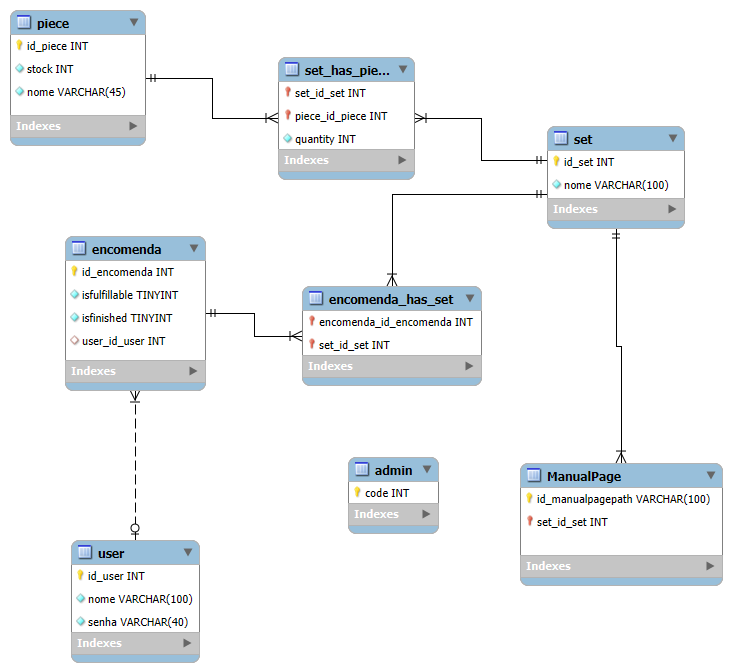
\includegraphics[width=\textwidth]{images/modelologico.png}
            \caption{Modelo lógico}
            \label{fig:modelologico}
        \end{figure}

    \newpage
    \section{Descrição de Elementos e seus Relacionamentos}
    Para melhor compreensão do modelo lógico da base de dados apresentámos duas tabelas para ajudar na perceção das entidades e relacionamentos da mesma.
    \begin{table}[h!]
    \centering
    \renewcommand{\arraystretch}{1.5} % Ajusta o espaçamento entre as linhas
    \begin{tabular}{|m{3cm}|m{6cm}|m{6cm}|}
        \hline
        \rowcolor{gray!28} % Cor de fundo da linha de cabeçalho
        \textbf{Entidade} & \textbf{Descrição} & \textbf{Ocorrência} \\ \hline
        \textbf{User} & Descrição geral para os que usam a aplicação na linha de produção & Cada user pode processar uma encomenda. \\ \hline
        \textbf{Encomenda} & Descrição geral para os pedidos vindos do departamento de gestão que contém os Sets a produzir para cada um. & Os users processam uma encomenda de cada vez, no caso produzem o Set dessa mesma encomenda. \\ \hline
        \textbf{Set} & Descrição geral para o produto que é produzido nas linhas de montagem. & Cada user vai produzir estes Sets consoante o que é pedido na encomenda. \\ \hline
        \textbf{Piece} & Descrição geral para o que compõe um Set. & O user vai usar este objeto para produzir os Sets, tendo sempre em atenção o stock do objeto. \\ \hline
        \textbf{ManualPage} & Descrição geral para uma instrução de montagem do Set. & Cada Set terá a si associado várias páginas que demonstrarão como este é produzido. \\ \hline
        \textbf{Admin} & Descrição geral para os códigos que serão usados para validar ações na aplicação que são identificadas como ações de administrador. & Cada código de administrador vai ser usado por um user identificado pela diração da empresa, para executar funções de administrador na aplicação. \\ \hline
    \end{tabular}
    \caption{Identificação das entidades}
    \label{tab:identificacao_entidades}
\end{table}
\newpage

\begin{table}[ht]
    \centering
    \begin{tabular}{|c|c|c|c|c|c|}
        \hline
        \rowcolor{gray!28}
        \textbf{Entidade} & \textbf{Multiplicidade} & \textbf{Relacionamento} & \textbf{Multiplicidade} & \textbf{Entidade} \\ \hline
        User            & 0..1                   & processa                     & N                   & Encomenda            \\ \hline
        Encomenda        & N                   & possui               & M                   & Set         \\ \hline
        Set         & N                   & possui              & M                   & Piece             \\ \hline
        Set           & 1                   & orientado              & N                   & ManualPage             \\ \hline
    \end{tabular}
    \caption{Relacionamento entre entidades}
    \label{tab:relacionamento_entidades}
\end{table}

    A entidade "Admin" não tem nenhum relacionamento, sendo assim uma tabela isolada, devido a não interagir com nenhuma outra entidade por não ser necessário. Esta entidade é apenas utilizada para armazenar as chaves de administrador no sistema, que vão ser utilizadas por certos funcionários definidos pela direção da empresa para efetuar ações de administrador na aplicação.


        

%==========================================================================
% END #4 - CONCEÇAO DO SISTEMA DE DADOS
%==========================================================================
